\documentclass{iagtese} 		% declara��o da classe iagtese com
						% padr�es de formata��o.
						%	
%\documentclass{iagtese_en}	% declara��o da classe iagtese em
						% ingles. Para escrever a tese em 
						% ingles, descomente esta linha e 
						% comente a linha anterior.
						%				%	
%\hypercolor				% links coloridos para a versao
						% on line da tese. Para usar esta
						% opcao descomente esta linha.
						% 	
\begin{document}			% in�cio do documento
						% 				
\institution{Universidade de S�o Paulo \\ Instituto de Astronomia, Geof�sica e Ci�ncias Atmosf�ricas \\ Departamento de Astronomia}

\title{T�tulo do trabalho}

\translator{{Tese/Disserta��o apresentada ao Departamento de Astronomia do Instituto de Astronomia, Geof�sica e Ci�ncias Atmosf�ricas da Universidade de S�o Paulo como requisito parcial para a obten��o do t�tulo de Mestre/{}Doutor em Ci�ncias.\\ \\
�rea de Concentra��o: Astronomia\\
Orientador(a): Prof.($^{\rm a}$) Dr.($^{\rm a}$) Orientador(a)}}

\author{Autor}

\date{S�o Paulo \ano}
			% arquivo para inserir a capa
						%
\pagestyle{empty}			% padr�o de formata��o para parte
						% inicial do texto
						%
\maketitle					% 
						%
\Dedicatoria				%
\hfill
\vfill
\hfill{\it{sua dedicatoria aqui!}}
\vspace{2cm}


		%
						% componentes iniciais do trabalho
\Agradecimentos			%
� minha fam�lia;

� fulana;

� orientadora;

Aos pesquisadores;

� Professora;

Aos colegas: 1, 2, 3 e 4

� FAPESP, pelo apoio financeiro, sob o projeto n$^o$: 6666/6666;

�s Institui��es

\vfill

\begin{flushleft}
\rule{6cm}{0.5pt}\\
{\footnotesize{Esta tese/disserta��o foi escrita em \LaTeX{} com a classe IAGTESE, para teses e disserta��es do IAG.}}
\end{flushleft}
	% caso n�o queira adicionar algum
						% deles, simplesmente remova as
						% linhas correspondentes.
						%
\Epigrafe					%  
\vfill
\begin{flushright}

``\textit{frase bonita 01}''\\

\vspace{0.4cm}

Autor da frase bonita 01

\end{flushright}

\vspace{0.5cm}

\begin{flushright}

``\textit{frase bonita 02}''\\

\vspace{0.4cm}

Autor da frase bonita 02

\end{flushright}

\vspace{2cm}
		%
						%
\Resumo					%
Resumo
		%
						%
\Abstract					%
Abstract
		%
						%
\listoffigures 				% lista de figuras (opcional)
\listoftables 				% lista de tabelas (opcional)
\tableofcontents 			% sum�rio
						%
\cleardoublepage			%
\pagestyle{fancy}			% formata��o para corpo do texto
						%
\chapter{Introdução}
\section{Considerações Iniciais}
\par{A grafita, um mineral de relevância crescente no panorama tecnológico e industrial, destaca-se por suas propriedades únicas e aplicações versáteis, desde o desenvolvimento de nanomateriais, como o grafeno, até seu uso em produtos industriais diversos. Este projeto de pesquisa foca na exploração de jazidas de grafita utilizando técnicas avançadas de aprendizado de máquina e sensoriamento remoto, concentrando-se no sistema de nappes de Socorro-Guaxupé.}

\par{Exploramos como os métodos geofísicos, em conjunto com o processamento de dados aerogeofísicos, podem ser utilizados para identificar padrões associados à mineralização de grafita. O objetivo é desenvolver um modelo preditivo robusto que melhore a eficiência da prospecção mineral e a gestão dos recursos naturais.}

\par{Esta pesquisa se insere em um contexto onde a demanda por grafita está em ascensão devido às suas aplicações em tecnologias emergentes. A grafita é amplamente distribuída em diversos tipos de rochas, mas a identificação de depósitos economicamente viáveis é um desafio que requer abordagens inovadoras. A integração de dados geofísicos com técnicas de aprendizado de máquina apresenta uma oportunidade única para abordar essa questão, potencializando a identificação de áreas promissoras para exploração mineral.}
		%
\chapter{Base de dados}\label{database}

Base de dados. Citar figura \ref{identificador}.

\begin{figure}[!ht]
\begin{center}
\setcaptionmargin{1cm}
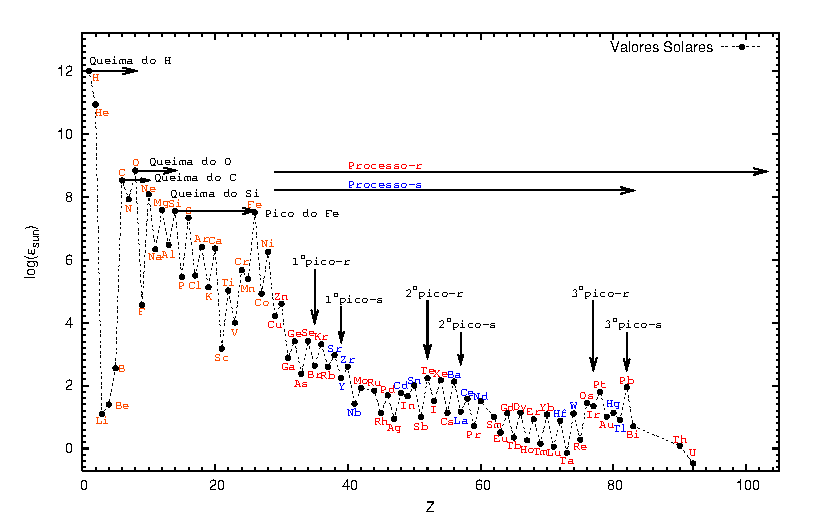
\includegraphics[width=1.0 \columnwidth,angle=0]{fig/solar_grevesse.eps}
\caption[Resumo da legenda da figura (aparece na lista de figuras)]{Legenda da figura.} 
\label{identificador}
\end{center}
\end{figure}


\begin{center}
\setcaptionmargin{1cm}
\scriptsize
\begin{longtable}{lcccc}
\caption[Resumo da legenda da tabela (aparece na lista de figuras)]{Exemplo de tabela feita com o longtable.}\\
\hline \hline \\[-2ex]
\multicolumn{1}{c}{Coluna1} &
\multicolumn{1}{c}{Coluna2} &
\multicolumn{1}{c}{Coluna3} &
\multicolumn{1}{c}{Coluna4} &
\multicolumn{1}{c}{Coluna5} 

\\[0.5ex] \hline
\\[-1.8ex]

\endfirsthead

\multicolumn{5}{c}{\footnotesize{{\slshape{{\tablename} \thetable{}}} - Continua��o}}\\[0.5ex]

\hline \hline\\[-2ex]

\multicolumn{1}{c}{Coluna1} &
\multicolumn{1}{c}{Coluna2} &
\multicolumn{1}{c}{Coluna3} &
\multicolumn{1}{c}{Coluna4} &
\multicolumn{1}{c}{Coluna5} 

\\[0.5ex] \hline
\\[-1.8ex]

\endhead

\multicolumn{3}{l}{{\footnotesize{Continua na pr�xima p�gina\ldots}}}\\
\endfoot
\hline

\endlastfoot

1 & 2 & 3 & 4 & 5 \\
6 & 7 & 8 & 9 & 10\\

\label{tabela_com_longtable}
\end{longtable}
\end{center}


    	% inserir os cap�tulos do seu
\chapter{An�lise}


An�lise
		% trabalho.
% Conclusão
\setlength{\fboxsep}{1cm}% Espaçamento interno do fbox
\fbox{% Cria um box ao redor do texto
    \parbox{\textwidth}{% Permite o controle de parágrafo dentro do fbox
        \setlength{\parindent}{1.5cm} % Define a identação dos parágrafos
        \fontsize{30}{36}\selectfont % Ajusta o tamanho da fonte e o espaçamento de linha
        \textbf{Conclusão}\\

\par{
    O desenvolvimento deste projeto evidencia a importância da sinergia entre dados geológicos e inteligência artificial, apresentando um protótipo promissor que aguarda validação em ambientes de supercomputação. Esperamos que a divulgação desta iniciativa inspire a colaboração, não apenas para refinamento e ampliação do modelo existente, mas também para explorar seu pleno potencial em análises preditivas avançadas de mapeamento geológico. 
}\\

} % Fecha o parbox
} % Fecha o fbox
		% 
       						%
						%
%\begin{thebibliography}{99}	% refer�ncias bibliogr�ficas (d�
%\bibitem{Quireza et al. 2007}{quireza}Quireza C., Rocha-Pinto H. J., Maciel W. J., 2007, A\&A, 475, 217

\bibitem[Aoki et al.(2001)]{2001ApJ...561..346A} Aoki, W., Ryan, S. G., Norris, J. E., Beers, T. C., Ando, H., Iwamoto, N., Kajino, T., Mathews, G. J., \& Fujimoto, M. Y. 2001, ApJ 561, 346

\bibitem[Aoki et al.(2002)]{2002ApJ...580.1149A} Aoki, W., Ryan, S. G., Norris, J. E., Beers, T. C., Ando, H., \& Tsangarides, S. 2002, ApJ 580, 1149 

\bibitem[Wasserburg et al. (1994)]{1994ApJ...424..412W} Wasserburg, G. J., Busso, M., Gallino, R., \& Raiteri, C. M. 1994, ApJ 424, 412
 	% prefer�ncia ao bibTeX).
%\end{thebibliography}		% caso n�o use o bibTeX, remova os
						% comentarios das tr�s linhas
						% e comente a linha \bibliography
						%
\bibliography{tex/bibliografia}	% bibliografia utilizando bibTeX,
						% referente ao arquivo
						% bibliografia.bib na pasta tex/
						%
\begin{apendice}			% inicio do ambiente apendice
\chapter{t�tulo do ap�ndice 01}\label{ap01}

\section{subt�tulo 01}\label{subap01}

\chapter{t�tulo do ap�ndice 02}\label{ap02}
		% texto referente ao apendice
\end{apendice}				% fim do ambiente apendice. caso
						% nao utilize apendice, remova as
						% 3 linhas de comando.
						%
\end{document}				% fim do arquivo
